\section {Problem Introduction}
In the traditional Internet architecture, a server handles incoming client requests.  This is referred to as the client-server paradigm.  The bottleneck in such systems tends to be the bandwidth at the server \cite{coopnet}, as this bandwidth is split $N$ ways among the accessing clients (see Fig. \ref{fig:traditional_http}).  When an increasing number of users access a web page, that page therefore loads more and more slowly.  This predicament is common, and occurs whenever server bandwidth is low, a server experiences a spike in load, or when clients download very large files.  A dramatic example of this problem is the ``slashdot" effect, in which a sudden ``flash crowd" of unanticipated clients may suddenly request certain pages, overwhelming the unexpectant server.  This can happen when sites are suddenly linked to by popular sites, such as slashdot.com.  These situations cause web servers to become overwhelmed and web users to have a less than favorable experience.

This problem is most commonly solved by distributing the load among a set of servers that mirror the content of the original server (see Fig. \ref{fig:server_only}).  A company establishes mirrors by locating a set of servers in many different places on the Internet, then automatically redirecting clients to these servers thus distributing the load to the various edge servers to provide better performance for users.  An example of this is the commercial CDN run by Akamai \cite{akamai}, which is employed by Apple to distribute their popular program iTunes\texttrademark.  This solution requires a dedicated pool of servers to provide the extra bandwidth, which can be expensive.  Not all sites can afford a CDN, and mirrors require cooperation, configuration, maintenance, and bandwidth.

As an alternative, many web sites are relying on \emph{peer-to-peer content distribution}, or \emph{swarming}, with BitTorrent.  In BitTorrent, clients download only some blocks of a file from a central server, and get the other blocks from their peers in the system.  While a client participates in BitTorrent, it is both downloading the blocks it needs and uploading the blocks it has to other peers (see Fig. \ref{fig:normal_swarm}).  Peer-to-peer content distribution enables a web server to serve a large file to large numbers of users without overloading its server bandwidth \cite{zappala}. Swarming protocols like BitTorrent \cite{cohen} or Slurpie \cite{slurpie} have been shown to even decrease download time per peer as the number of peers increases. 
% I put these figures here (later) in an effort to avoid having it at the top of the first page, which is a little ugly
\begin{figure}
\begin{center}
   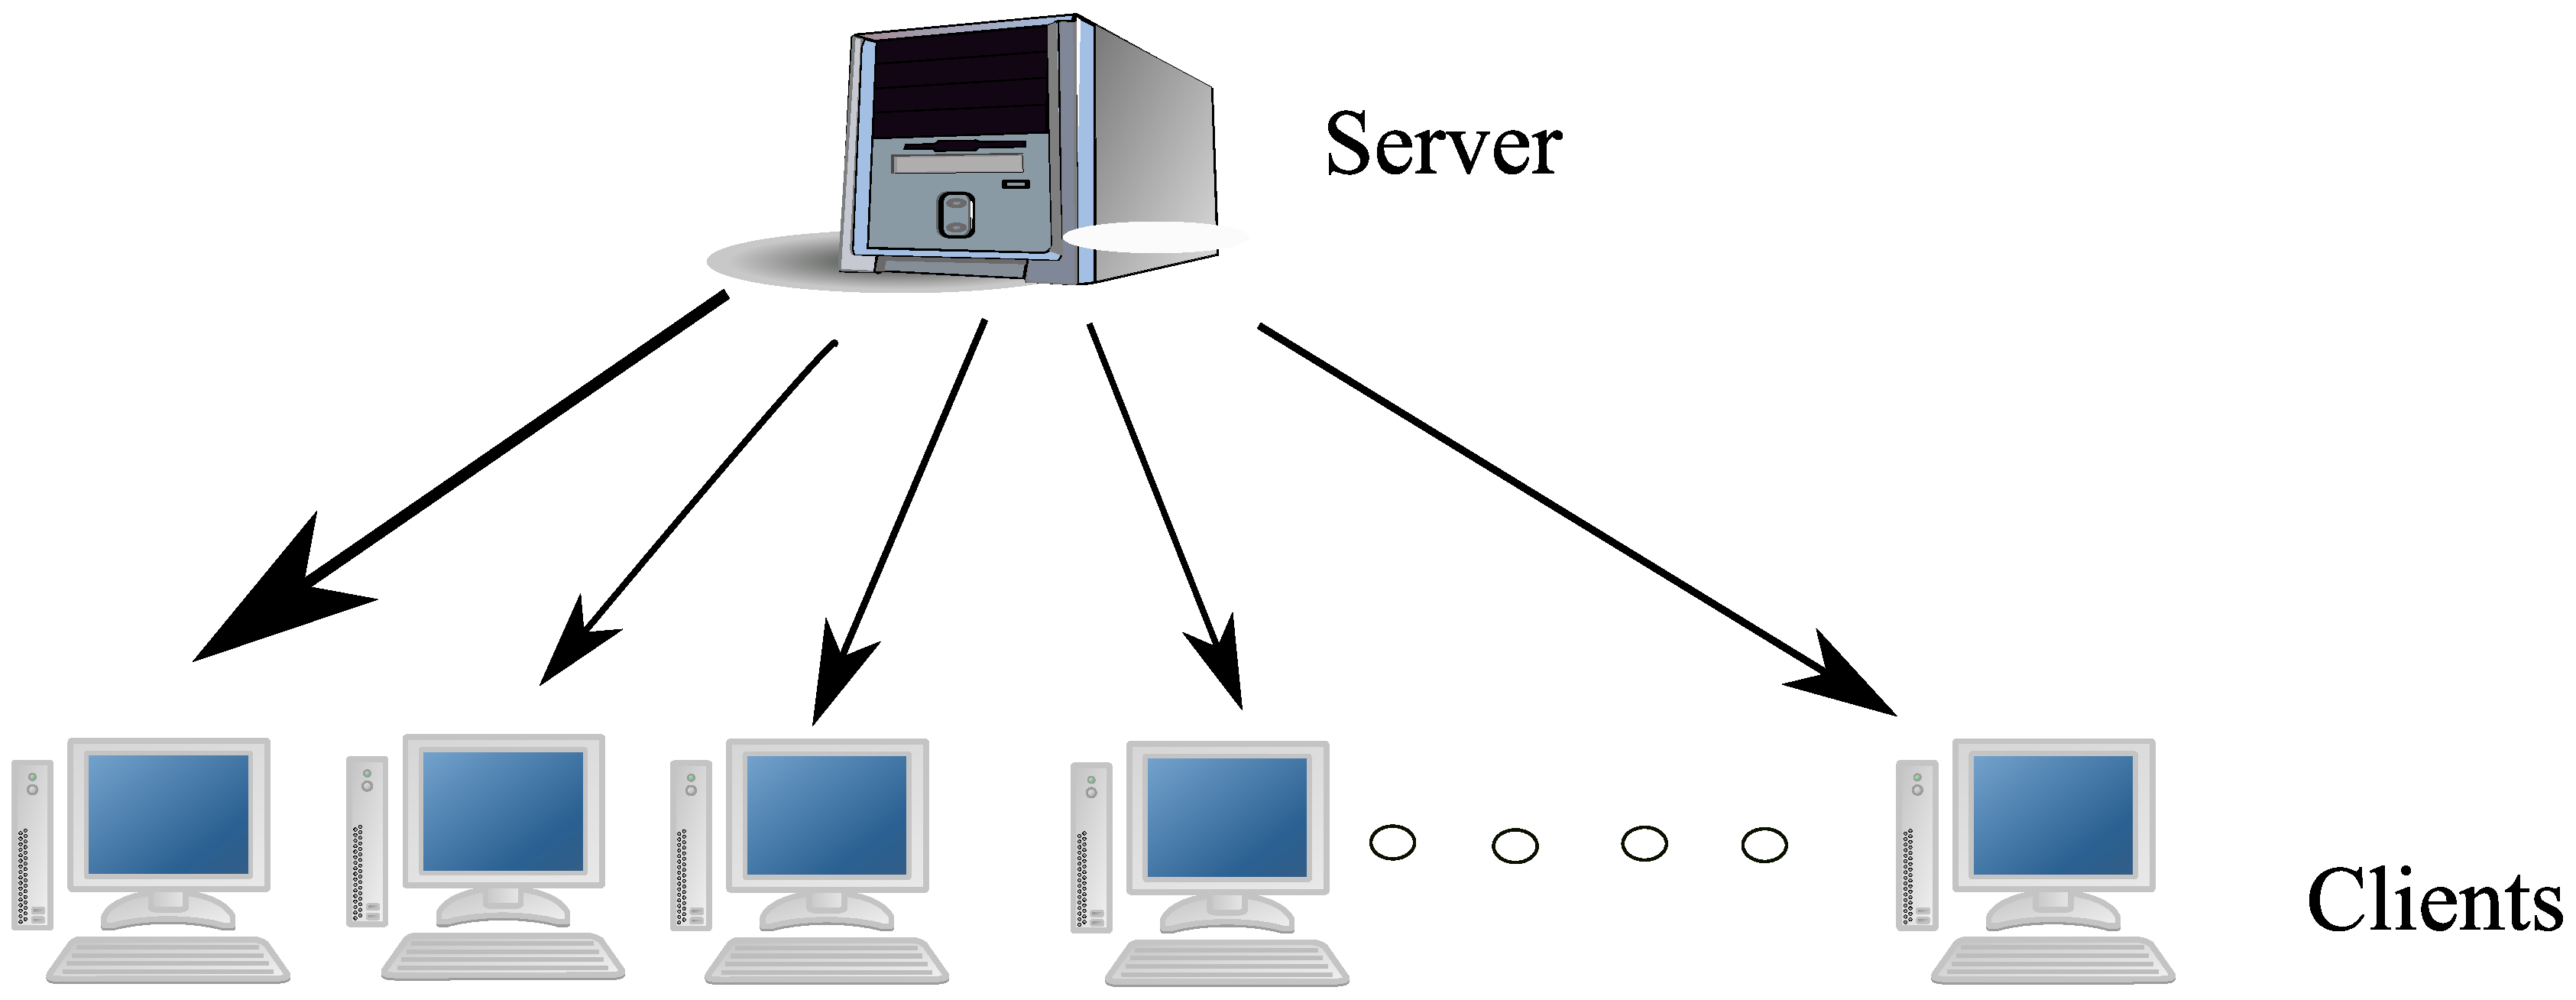
\includegraphics[width=11cm]{pics/traditional_http.eps}
    \caption{Traditional HTTP download}
 \label{fig:traditional_http}
 \end{center}
\end{figure}
\begin{figure}
    \centering
  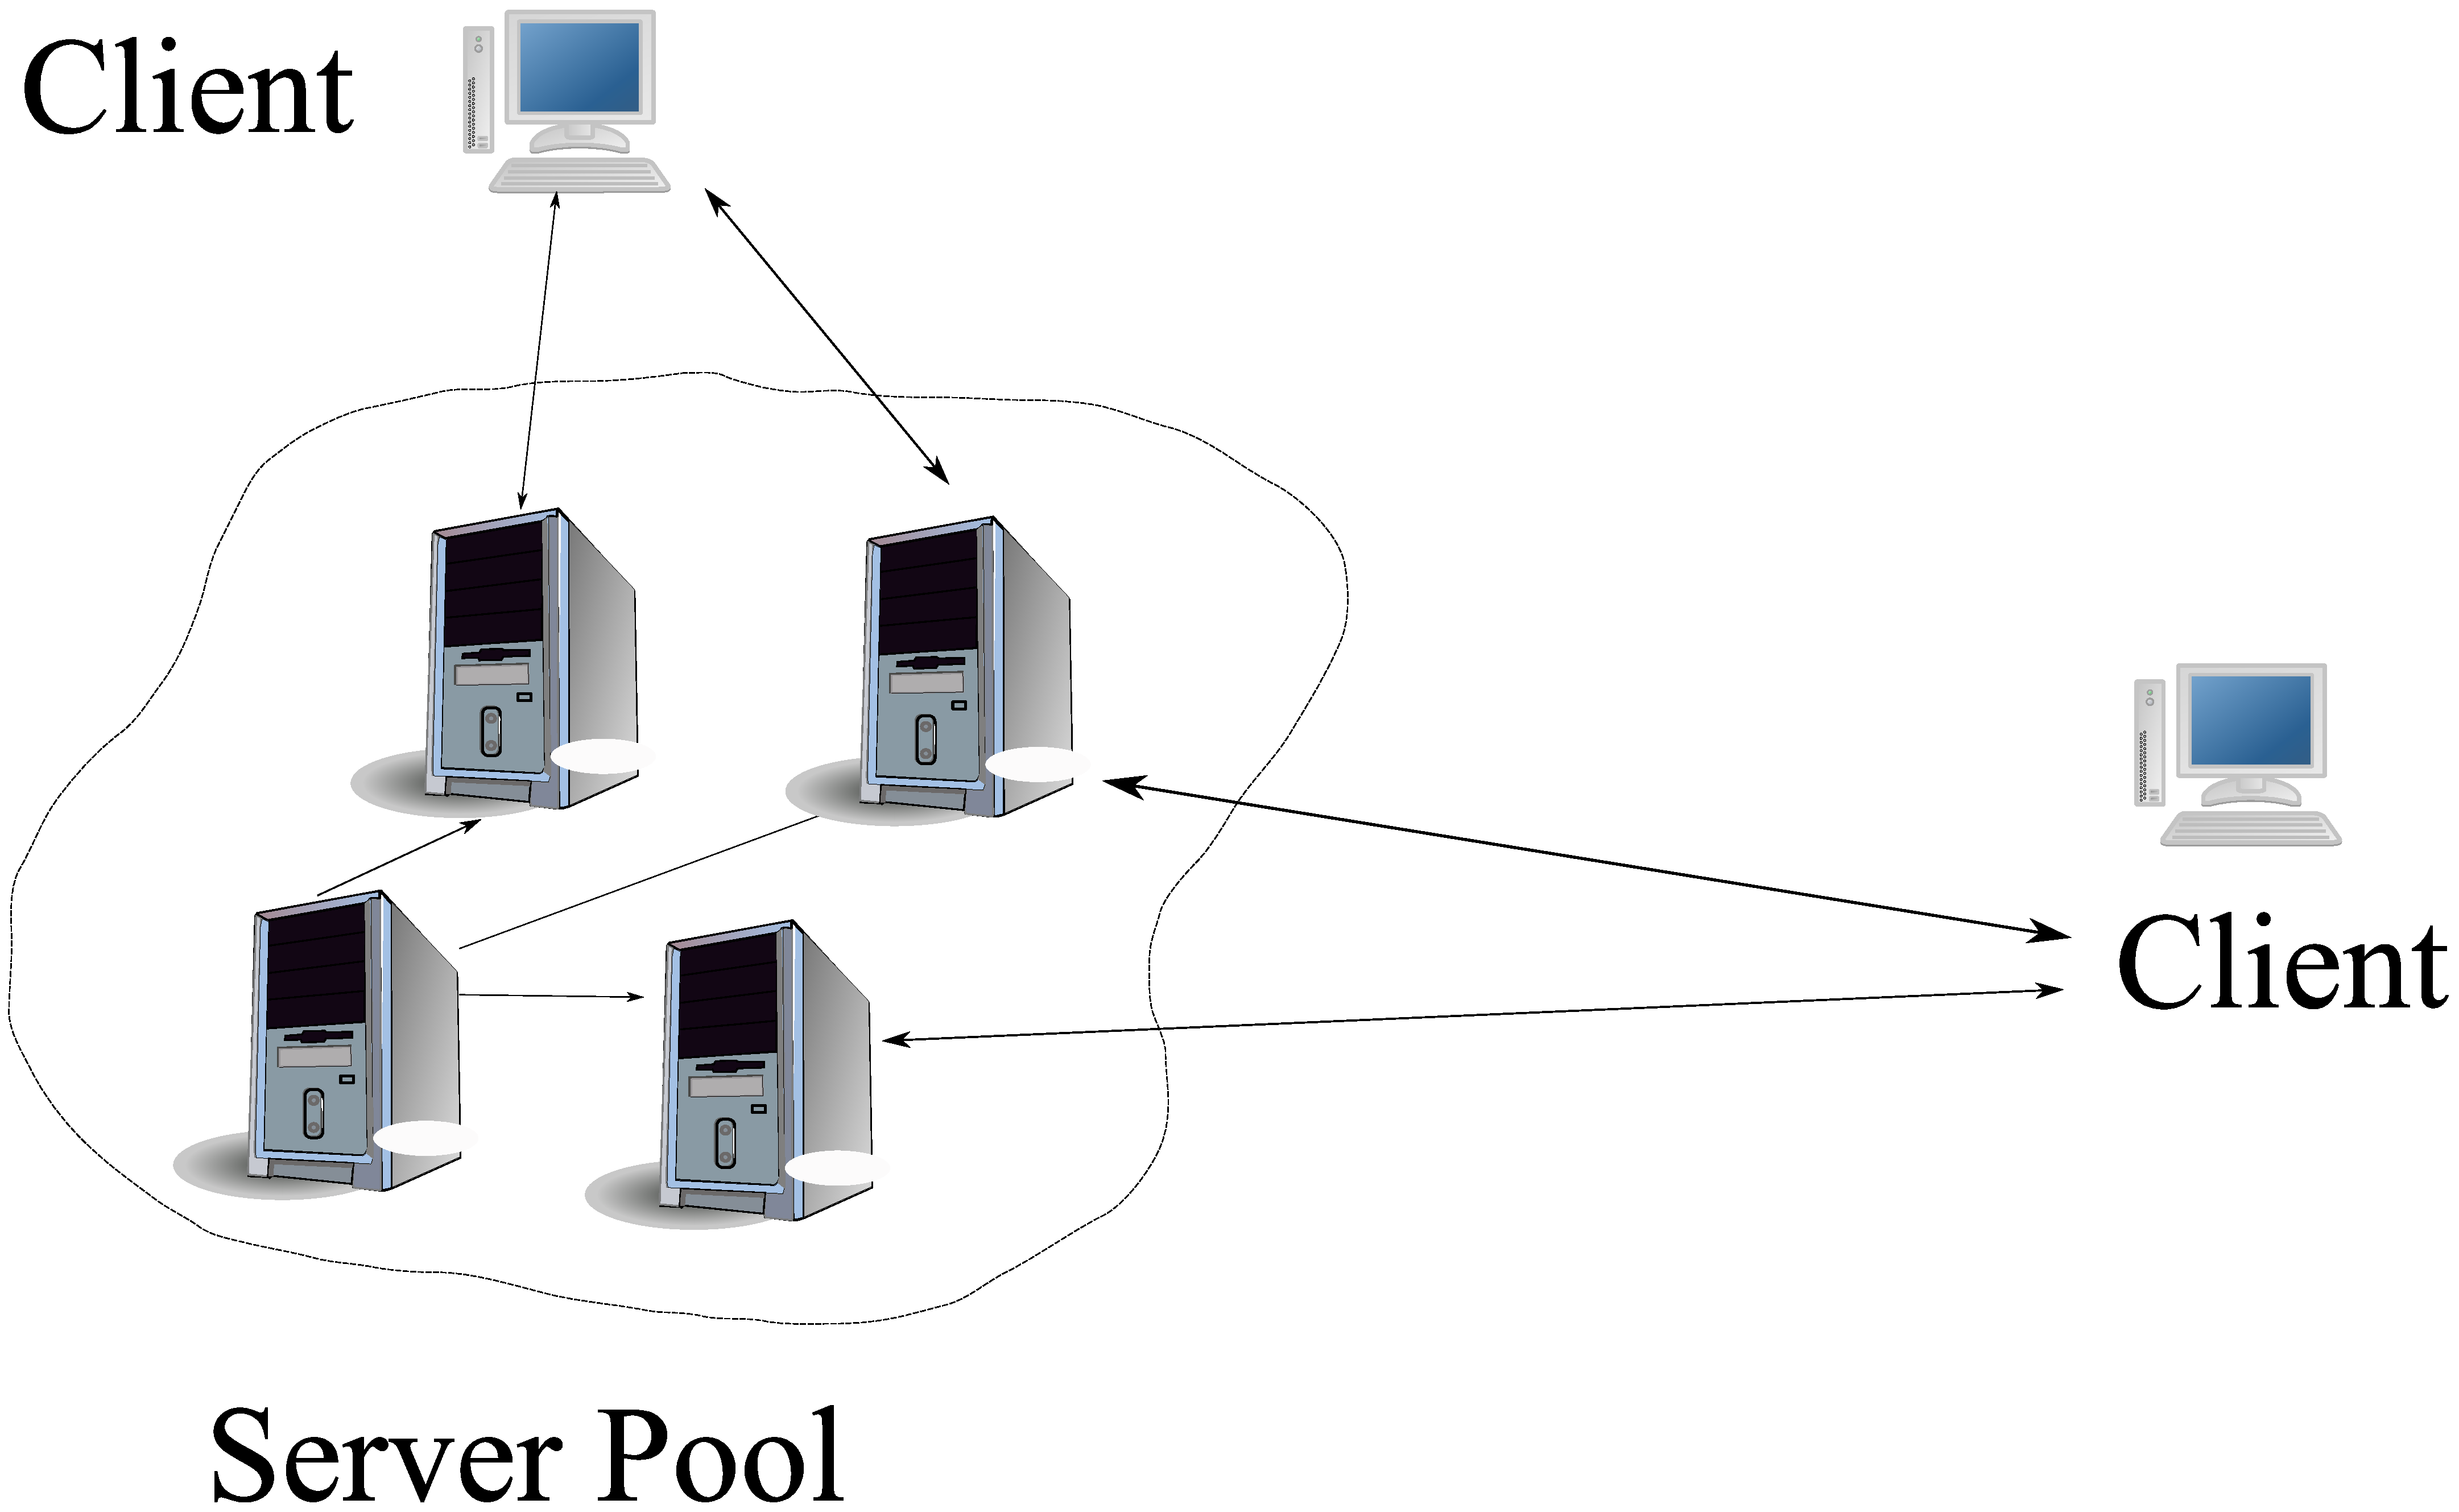
\includegraphics[width=8cm]{pics/server_side_only.eps}
  \caption{Server CDN example}
  \label{fig:server_only}
\end{figure}   
\begin{figure}
 \centering
 
\includegraphics[width=4.5cm]{pics/normal_swarm.eps}
 \caption{Swarming example.  Arrows represent block exchanges.}
 \label{fig:normal_swarm}
\end{figure}

BitTorrent splits files into blocks and connects peers sharing them in a mostly distributed fashion.  To accomplish a BitTorrent download, peers must first locate a file with a ``.torrent'' extension from an out of band source such as a  web server.  This file lists a target file's size, MD5 hashes of the different blocks of the file (for integrity verification), and the IP address of a tracker for that file.  This tracker is a machine which helps connect the peers to each another.  Peers contact the tracker and receive a random list of other peers who are currently downloading the file.  They  then establish connections and begin sharing and receiving blocks with their new neighbors.  Peers in BitTorrent tend to share with peers that also share with them, which creates an incentive for cooperation in the system, referred to as Tit-For-Tat.  Finally, when a peer has downloaded the entire file, it may linger in the system, acting as a ``seed" and uploading file blocks altruistically. 

%->final:Peers choose which blocks to download based on a "rarest first" policy.  This enables rare parts of the file to propagate quickly in the download swarm. 

%->final:BitTorrent, for the download of the last block of a file, uses a kind of 'many peers downloading the same blocks.  It requests the last block simultaneously from many peers, so that if one peer is transmitting it very slowly, they will be quickly passed by one of the faster seeds, and thus download it quickly.

BitTorrent is inappropriate for serving all the files in a web site.  It is designed for large files and is not easily used to serve all files from a web server.  For every file that is to be shared a .torrent file must be created, and a tracker established for that file.  This type of manual configuration is difficult to repeat for an entire web site.  Also, swarms are formed on a per file basis, so it is not possible for a peer in one swarm to find a different file among its peers in the swarm.  BitTorrent also uses Tit-For-Tat incentives to share blocks of the same file, which is not appropriate for multiple small file downloads, and causes a longer boot-strapping time.  

Ideally, a web server could automatically serve all its files using peer-to-peer file transfer and would automatically transition to peer-to-peer downloads based on the load it experiences.  This has been proposed before, but would require that all web servers and clients would use a defined peer-to-peer protocol.  Instead, this thesis proposes modifying only web clients so that they can automatically transition to peer-to-peer download for all files on a web server.  They will be able to communicate with other modified web clients to get faster downloads, which in turn will provide an incentive to adopt this protocol.

% in the real thesis I want to mention the BitTorrent DHt and trackerless..... -> One problem with BitTorrent is that it relies on a central tracker to rendezvous available peers.  This tracker can become overwhelmed like any other web server, or can go off-line, thus crippling the ability of peers to locate each other.  To combat this, BitTorrent itself and the recent BitTorrent client Azureus \cite{azureus} have recently integrated optional `trackerless' modes, in which peers bypass the tracker and locate other peers via a query to a Distributed Hash Table (DHT).  DHTs are a distributed storage system with a basic API for the storage and lookup of $<key,value>$ pairs.  DHTs can perform these functions in $O(log(n))$ time, and are resilient to node failure, which makes relying on them for peer rendezvous more scalable than a centralized tracker.  This solution is currently used for discovering peers that are downloading a file, but not in discovering which peers have which blocks.  We feel that for small files, such as those present on the web site, that a block by block lookup system may be faster (with BitTorrent you look up peers, then blocks).  BitTorrent is mainly used for large files since it makes more sense, as there are more blocks that peers could trade.  It hence has a reputation for slow ramp up time (because of the tit-for-tat incentive policy).  This is not necessarily suitable for web content delivery.
%final: note that the .torrent file could get creamed...A second problem with BitTorrent is that it requires a manual setup of the `.torrent' file.  This limits the usefulness of BitTorrent, because a web site administrator must configure these for files that are large or that might become popular.  In addition, it requires every client to download the `.torrent' file from some central web server, which may be too high of a load, depending on the available bandwidth.   This problem also exists with the trackerless BitTorrent.  These problems limit its usefulness as an automatic web download system.  We therefore propose a system where peers attempt to download content, and if the origin server is slow they transition to a peer-to-peer system for content delivery.  This will be block-wise to ensure speed, and is described more fully in section \ref{section:solution}.


\section {Thesis Statement}\label{section:thesis}
A system of cooperating web clients can reduce load on a origin web server by automatically switching from client-server file transfer to peer-to-peer content delivery.  This system can provide fast download times for objects of many sizes, especially small files.  It should be equivalent in speed to BitTorrent for larger files, without requiring any manual configuration or participation from central web servers.

\section{Related Work}\label{section:related_work}
Much work has been done to distribute file downloading.  Solutions fall into three basic categories:  client-side protocols, client and server-side cooperative protocols, and server-side protocols.  Each category has certain trade-offs in terms of how ideal it is, in our context.

\subsection{Client-Side Only Protocols}
Protocols that use only client-side protocols can help alleviate flash crowds.  Client-side interaction typically involves peers self-organizing to help speed downloads.  These solutions require no change in the server software, which allows them to be implemented in participating clients without requiring web servers to be aware of the changes.  However, this requires that clients must self-organize without the help of a centralized server.

Shared web caches are an example of this type of system.  They provide stable solutions for peers by allowing them to download files from a shared cache \cite{coral} \cite{codeen}, though they may require some type of dedicated infrastructure of cache members.  Squirrel \cite{squirrel}, for instance, is a shared web cache designed for use on a local LAN.  Squirrel clients join a DHT and cache any files that map to their location in the DHT.  When a user requests a file, that user contacts the member of the local DHT who should be caching that file, and requests it.  If the member does not have a copy of the file, it first downloads it from the origin web server, then caches a copy and returns the result to the requesting user.  Squirrel does a good job of sharing the caches of participating members on a local LAN.  It does not offer an algorithm for transparent transition to p2p download, however, always relying on the proxy for static content.

CoDeen \cite{codeen} \cite{coblitz} is a distributed proxy, where participating members of the system act as a large web cache which is accessible to outside users.  It is the equivalent of a globally accessible, wide-scale version of Squirrel.  The load of caching objects is distributed among the different nodes so if one node goes down the entire system is not dramatically affected.
It works as follows:

1) Users set their Internet browser proxy to a nearby high bandwidth participant of CoDeen and request all files from it.

2) The proxy, upon receiving requests for a file, either returns the file from its cache, or retrieves it and returns it.  To retrieve a file, the proxy requests it from a live member of CoDeen that is the 'owner' of that file.  If the owner has it, it returns the file, otherwise it contacts the origin server and downloads, it then returns it.  Codeen also provides load balancing by performing heartbeat tests of its neighbors before requesting files from them.  

Similarly, in Coral \cite{coral}, participating members of a DHT act as a web cache.  Users who access this system are redirected (via HTTP redirect) to a close Coral member, which then searches for the file on the DHT, retrieves it, and forwards it on to the user.  Coral has a central point of failure in its DNS redirection system, in that it requires a central server to administer all requests for files.

These solutions have some advantages and disadvantages.  The advantages are that they reduce the load on the origin server, they load balance among cache members, and they are distributed over a wide area.  The disadvantages are that they are constrained to the number of participating proxies. They require an infrastructure of hosts who are willing to altruistically provide bandwidth, which is a rarity.  This means that for these systems, in extreme situations (load surpassing the bandwidth of the combined sum of computers), they would still become overburdened.  With our system this should not be a problem, as more peers in the system means that more peers will be available for uploading.  This also holds as in traditional web browsing much time is spent only reading pages, which time can be dedicated to uploading content to others at no cost.  Having an infrastructure also requires members of the DHT cache files for which they are not directly interested, and clients must choose a single static proxy that can become overloaded or go off-line.  Choosing a single proxy, even per file, is dangerous as it could become overloaded as network conditions change.  These systems also lack an algorithm for transition from traditional to peer-to-peer download.  They always return the cached copy, even if a request from the origin server would have been the fastest way to download the file.    

The effect of  flash crowds may also be alleviated by searching among a random subset of Internet peers for desired files.  PROOFS \cite{proofs} (P2P Randomized Overlays to Obviate Flash-crowd Symptoms) uses flooded search to allow peers to locate 'popular' or 'flash crowded' files from other peers who have previously downloaded the same.  The creators conjecture that files that are the subjects of a flash crowd are likely to be locatable among random sets of peers, since they are popular, hence their use of a random flood search.  The benefit of this system is that nodes need not maintain a structured search system (such as a DHT). However, not having a DHT for lookup makes searches more random and slightly less accurate, with potentially higher overhead.  PROOFS also does not include parallel downloads nor offer a protocol for automatic transition to a peer-to-peer solution.

Overall, client-side solutions alleviate flash-crowds well, though they are limited by the bandwidth of contributing members in certain cases. There also seems to be no automatic transition to peer-to-peer download.

\subsection{Server-side and Client-side Cooperative Protocols} 
Many file distribution protocols include some cooperation and previous knowledge between the server and client.  In these protocols clients typically access blocks of a file from the server and also from peers.  Server-side and client-side cooperative protocols basically fall into two categories: those used for web redirection, and those used to download single objects.  For web redirection, servers typically redirect clients to former clients that have downloaded files previously \cite{pseudoserving, coopnet}.  This allows a server to 'meter' its upload speeds and redirect peers, when appropriate, thus providing a backup strategy for over-loaded servers.  An example of this is the pseudo-server system \cite{pseudoserving}.  This style of protocol typically requires changes to both the server and client software, however, and the server could still become overloaded in extreme cases.

%Kept around because I hate to delete them: In the pseudo-server system \cite{pseudoserving, coopnet}, peers which contact a server offer to upload files they are requesting to other peers in exchange for the download of the file.  Peers basically promise to re-upload the file to some later peer that may contact the server. When the server later exceeds a certain load limit it redirects peers to the clients who have incurred a debt to the server (who then serve the file and hence become pseudo-servers).  This depends on trustworthy clients to repay their debts.

Some proposals incorporate the above web redirection, but also include swarming \cite{overhaul, webtorrent, onion}.  Swarming provides the benefit of scalable downloads of large files.  These protocols basically redirect peers to each other and also hand each a block of the file, then let the peers trade amongst themselves to create the entire file.  
OnionNetworks, for instance, proposes an extension to HTTP to allow HTTP response messages to include hashes of files and a list of peers from to which other peers may connect and download in a swarming fashion \cite{onion}.  
Several protocols simply initiate block-wise file distribution for arbitrary objects \cite{zappala, cohen, slurpie, mutualcast, fastreplica, avalanche, bullet_prime}.  BitTorrent, the most commonly used swarming protocol, was developed in 2001 by Bram Cohen \cite{cohen}.  Its major contribution (besides popularizing swarming) is the use of Tit-For-Tat to encourage sharing and discourage free-loading.  Swarming protocols are highly effective in response to flash crowds, effectively serving loads orders of magnitude higher than an ordinary web server \cite{zappala}.

Shark \cite{shark} is a file system prototype that allows clients to download blocks of files from nearby neighbors who have blocks already on their local machines. 
Shark is similar to our proposed system, except applied to files in a file system, not web objects.  It  requires a custom DHT for peer localization and proximity estimation, and a central server for hash values of files.  It also lacks HTTP integration and a switching mechanism.

These systems typically are used for downloading single, predetermined, static files.  They all therefore do a straight p2p transfer, without a transition mechanism from normal web download.

Some solutions seek to integrate HTTP clients with BitTorrent itself.  In these solutions a user is presented the option of downloading via HTTP or via BitTorrent (swarming), depending on which they think will give them the quicker download.  This provides a backup for overloaded servers.  To the users this requires a manual transfer from normal to swarming download.  The Osprey system \cite{osprey}, for example, is an ftp server that automatically generates .torrent files for all files in an ftp sub-directory, and integrates a BitTorrent tracker into the server software to handle the two types of requests.  Several other sites also offer .torrent files alongside normal (typically large) files, to allow users to manually use swarming in cases of high load.  These systems allow peers to manually switch to swarming if the server load becomes too high.  Dijjer \cite{dijjer} is a tool that automatically performs swarming downloads of any file.  If passed a url like http://dijjer.org/get/http://mysite.com/video.mov the request is intercepted by the Dijjer software, which performs a distributed download of the file.  One can also right-click on any arbitrary file and select 'download via Dijjer' for the same effect.  Dijjer contacts a quasi-DHT (similar to Freenet \cite{freenet}) for block hashes and downloads the blocks from random peers who cache these blocks.  Unfortunately, Dijjer lacks automation in the transition to download, and, as the Dijjer software is currently implemented, requires peers to cache material in which they were never interested.  

Overall, client and server side cooperation protocols work well at alleviating flash crowds, and some provide automation for transition to p2p delivery.  However, they require both the server and client to understand the protocol, which hinders their adoptability.  The biggest drawback of these protocols is that they are not transparent to the server.

\subsection{Server-side only Protocols}
Server-side only solutions typically create a pool of servers that mirror each others' content, helping to alleviate the impact of flash crowds \cite{backslash, dotSlash}.  In these systems, servers will cover for each other, so that if one becomes very crowded then the others will share the load with it until load decreases.  Backslash \cite{backslash} is one example.  In Backslash, when one server becomes overloaded it redirects requests and uploads necessary files to other servers for them to act as temporary mirrors, therefore relying on the volunteer hosts in the system.  

Overall, server-side systems still tend to be susceptible to flash crowds (albeit to a lesser extent), because of their collaboration, and are built to serve clients that are not p2p enabled, so offer no transition.


\section {Proposed Solution}\label{section:solution}
Our proposed solution emphasizes a client-only system that automatically switches from client-server to a peer-to-peer content delivery without any manual configuration for either clients or servers.  The goals for our system include:
\begin{enumerate}
\item It should be transparent to servers.  This allows the origin servers to remain unchanged, so end users can benefit immediately from the system.
\item It should appear transparent to users by automatically transitioning to peer-to-peer content delivery when the server is slow.
\item It should not require a dedicated special-purpose infrastructure.  Using a general-purpose infrastructure, coupled with a dependence on the clients for transferring blocks, makes this system easier and cheaper to deploy.
\item It should be non-intrusive, in that peers should not be required to cache blocks of files in which they were never interested.  Peers will avoid caching files they never downloaded, and will not be responsible for content they don't anticipate.  Users would also only be using heir upload bandwidth for files in which they are interested, encouraging participation and adoption.
\item It should be fast for small files.
\end{enumerate} 

Future goals might include ensuring the validity of files and providing explicit incentives.

The basic system will be to connect interested peers with one another via a DHT that stores peers lists.  A fundamental design decision is also whether to download the contents of blocks from peers or from the DHT itself; peers could store the block contents, and have the DHT serve as a lookup of peers, or could store the block contents on the DHT itself.  The trade-off is that having the blocks on the DHT puts more stress on the DHT and relies on members of the DHT for contributing bandwidth, which is intrusive.  Imagine for instance caching portions of a file on your personal computer which you never downloaded for yourself, and which you are then sharing with others.  Members of the DHT would thus intrusively cache information for which they are not interested.  We therefore choose the case of having peers register themselves on a DHT as being willing to serve blocks they own, and have clients download directly from peers.  This seems more indicative of a realistic web experience.

\input basic_algorithm

\subsection{Basic Algorithm}

In our protocol, a peer first tries to download the file from an origin web server.  If at some point one of the following conditions occurs, the download will switch to a peer-to-peer swarming download:
\begin{enumerate}
\item First the client waits a maximum amount of time $T$ after the start of a normal HTTP download for the first byte of data to arrive.  This allows the system to decide quickly whether the origin server is over-burdened and switch to peer-to-peer if needed.   
\item Once the client gets some data from the server, then it monitors whether the download rate falls below a certain fixed threshold $R$ bits per second over a window of time $w$.  If the origin server ever becomes slow, the client switches to peer-to-peer delivery.
\end{enumerate}

Once a client decides to switch to peer-to-peer downloading it will perform two steps.  First the client will calculate a hash value for the filename.  It will use this as a $key$ value in the DHT to retrieve a list of the blocks of the file.  The peer will then take each of the blocks' respective hash value as a $key$ to retrieve a list of peers who have the block and are willing to upload it.  The peer will choose one peer at random from the list, download the block from that peer, and then add itself to the list of those containing the block (see Fig. \ref{fig:download_all_steps}).  If there are no peers listed for a block, it will make a note in the DHT that it is accessing the origin server for that block, and download it using an HTTP Content-Range request from the origin server.  Peers will initiate this block-wise transfer for some $b$ blocks at a time.  If peers download a file previously unknown to the system, then the hash values for each block will be unknown.  In this case a peer will first make a note that they are accessing the origin server, for that block, then they will download it, calculate its hash value, and add themselves as the first peer in the list of those having that block.  This should accomplish a distributed download without any server knowledge or manual configuration.

\begin{figure*}
  \begin{center}
    \subfigure[Peer downloads list of blocks]{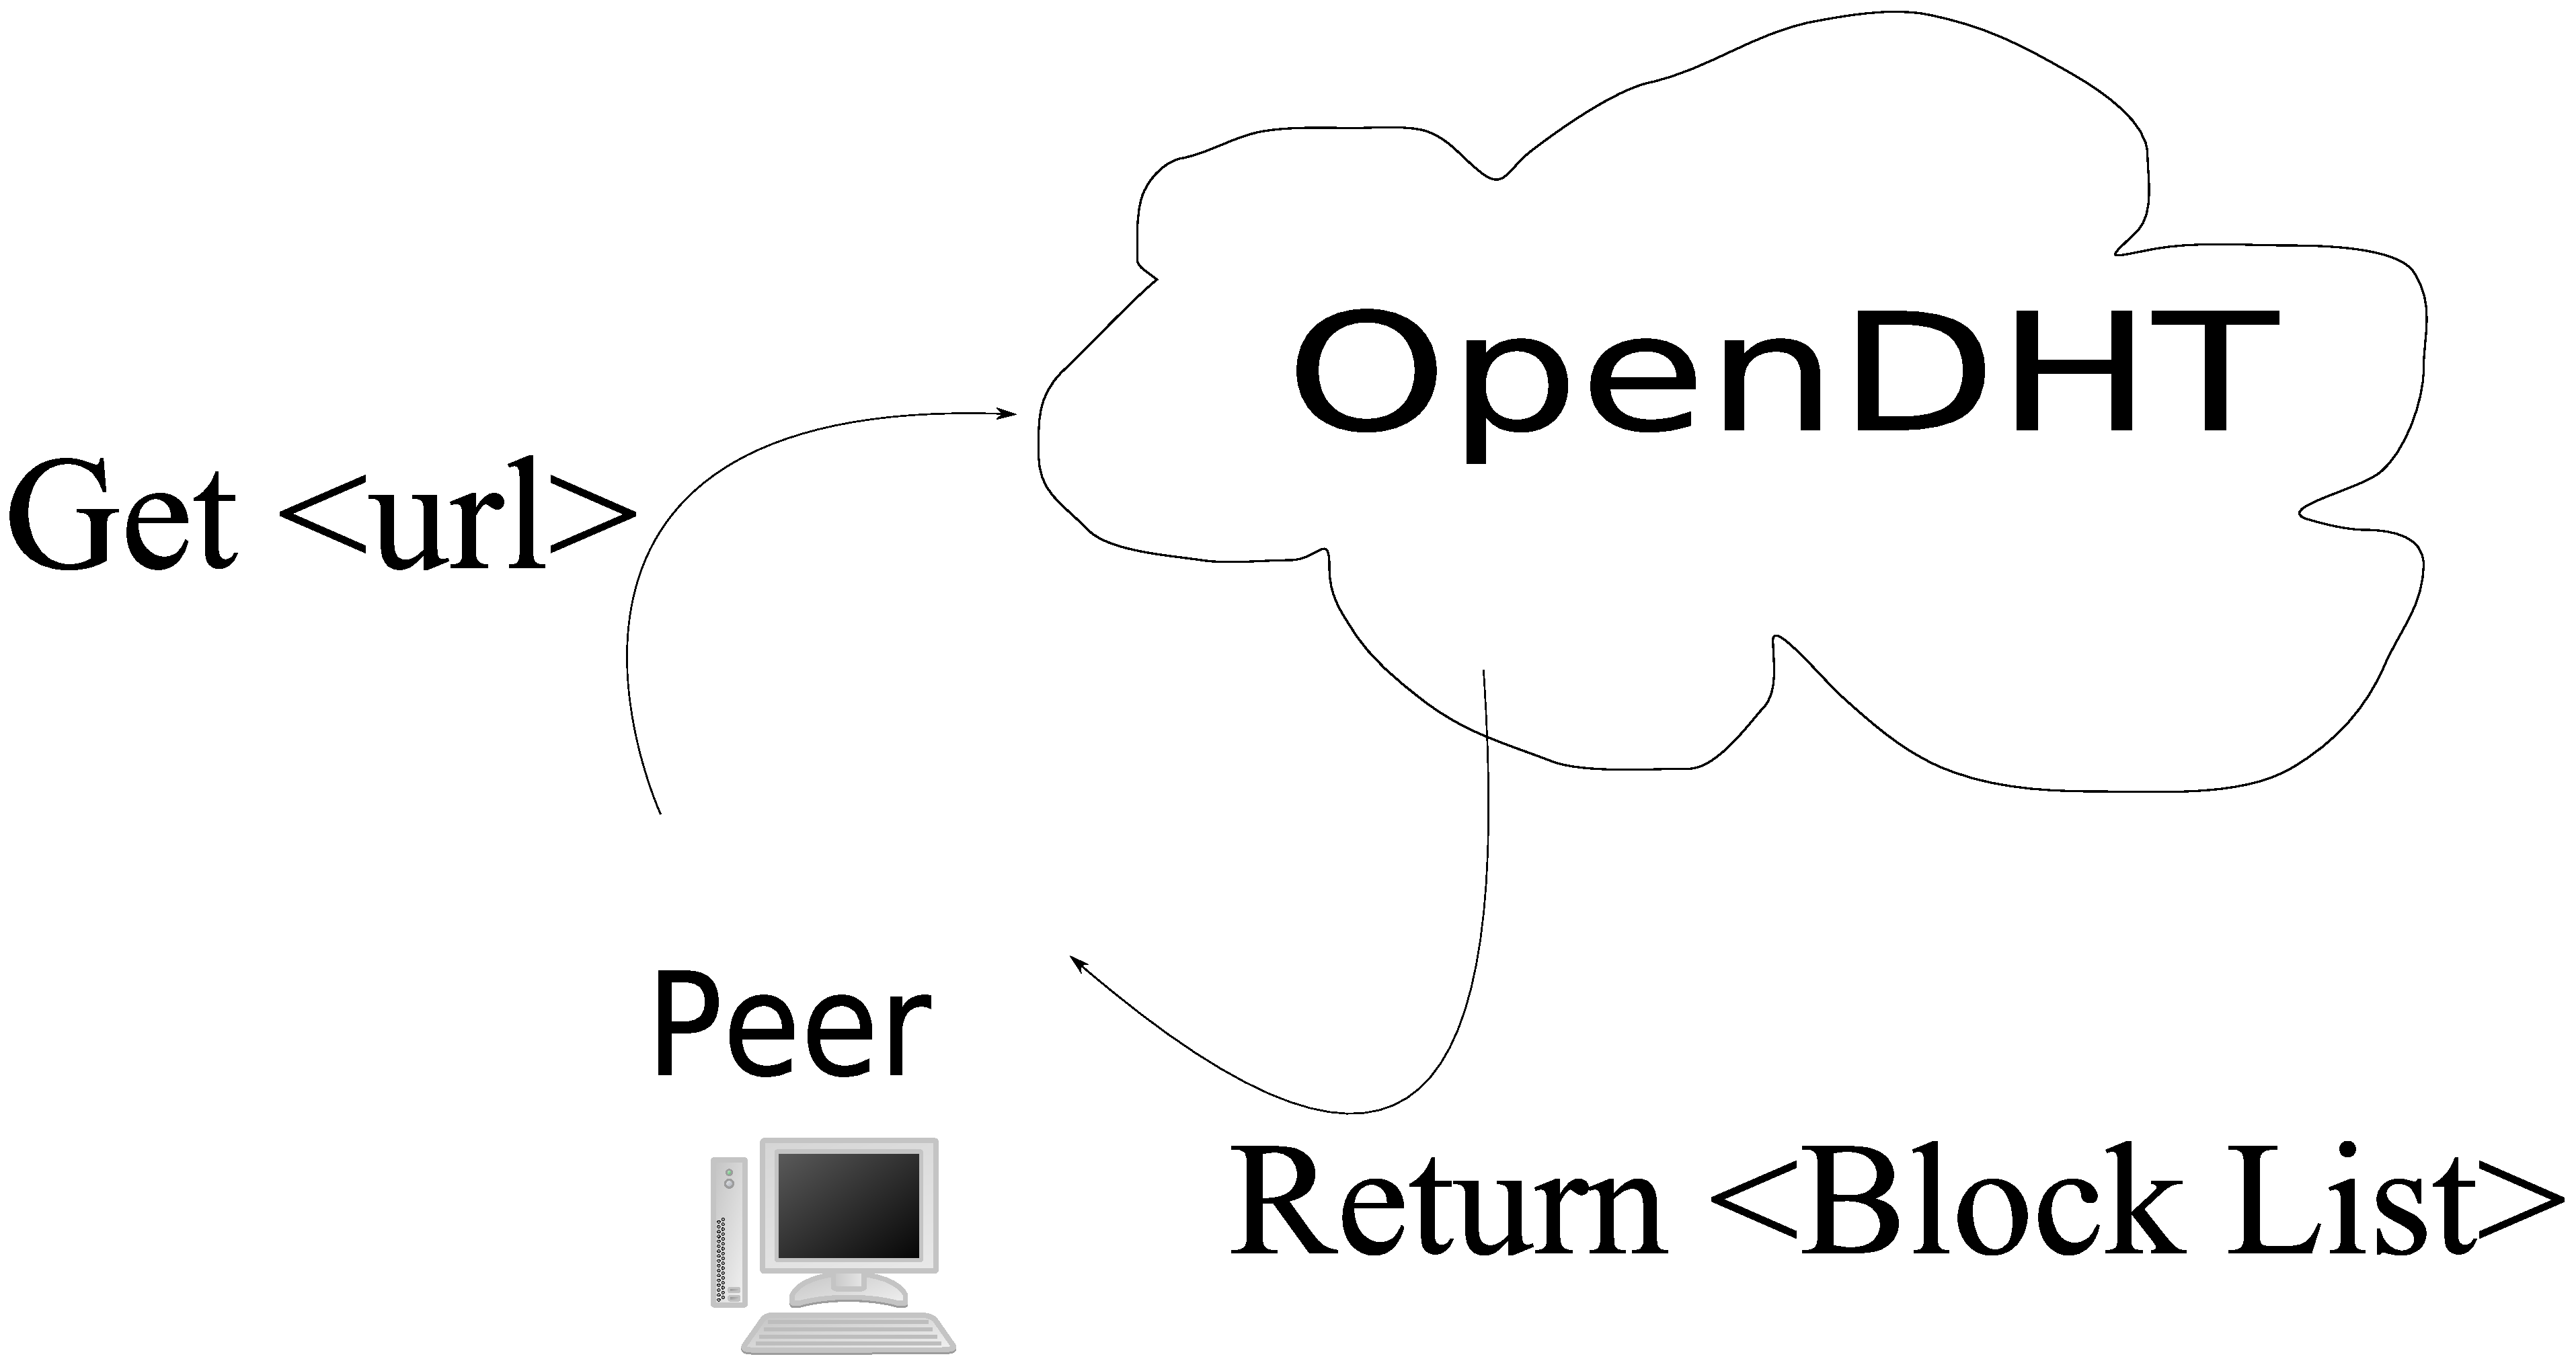
\includegraphics[width=7cm]{pics/peer_step_1.eps}}
    \subfigure[Peer downloads a list of peers which have a block]{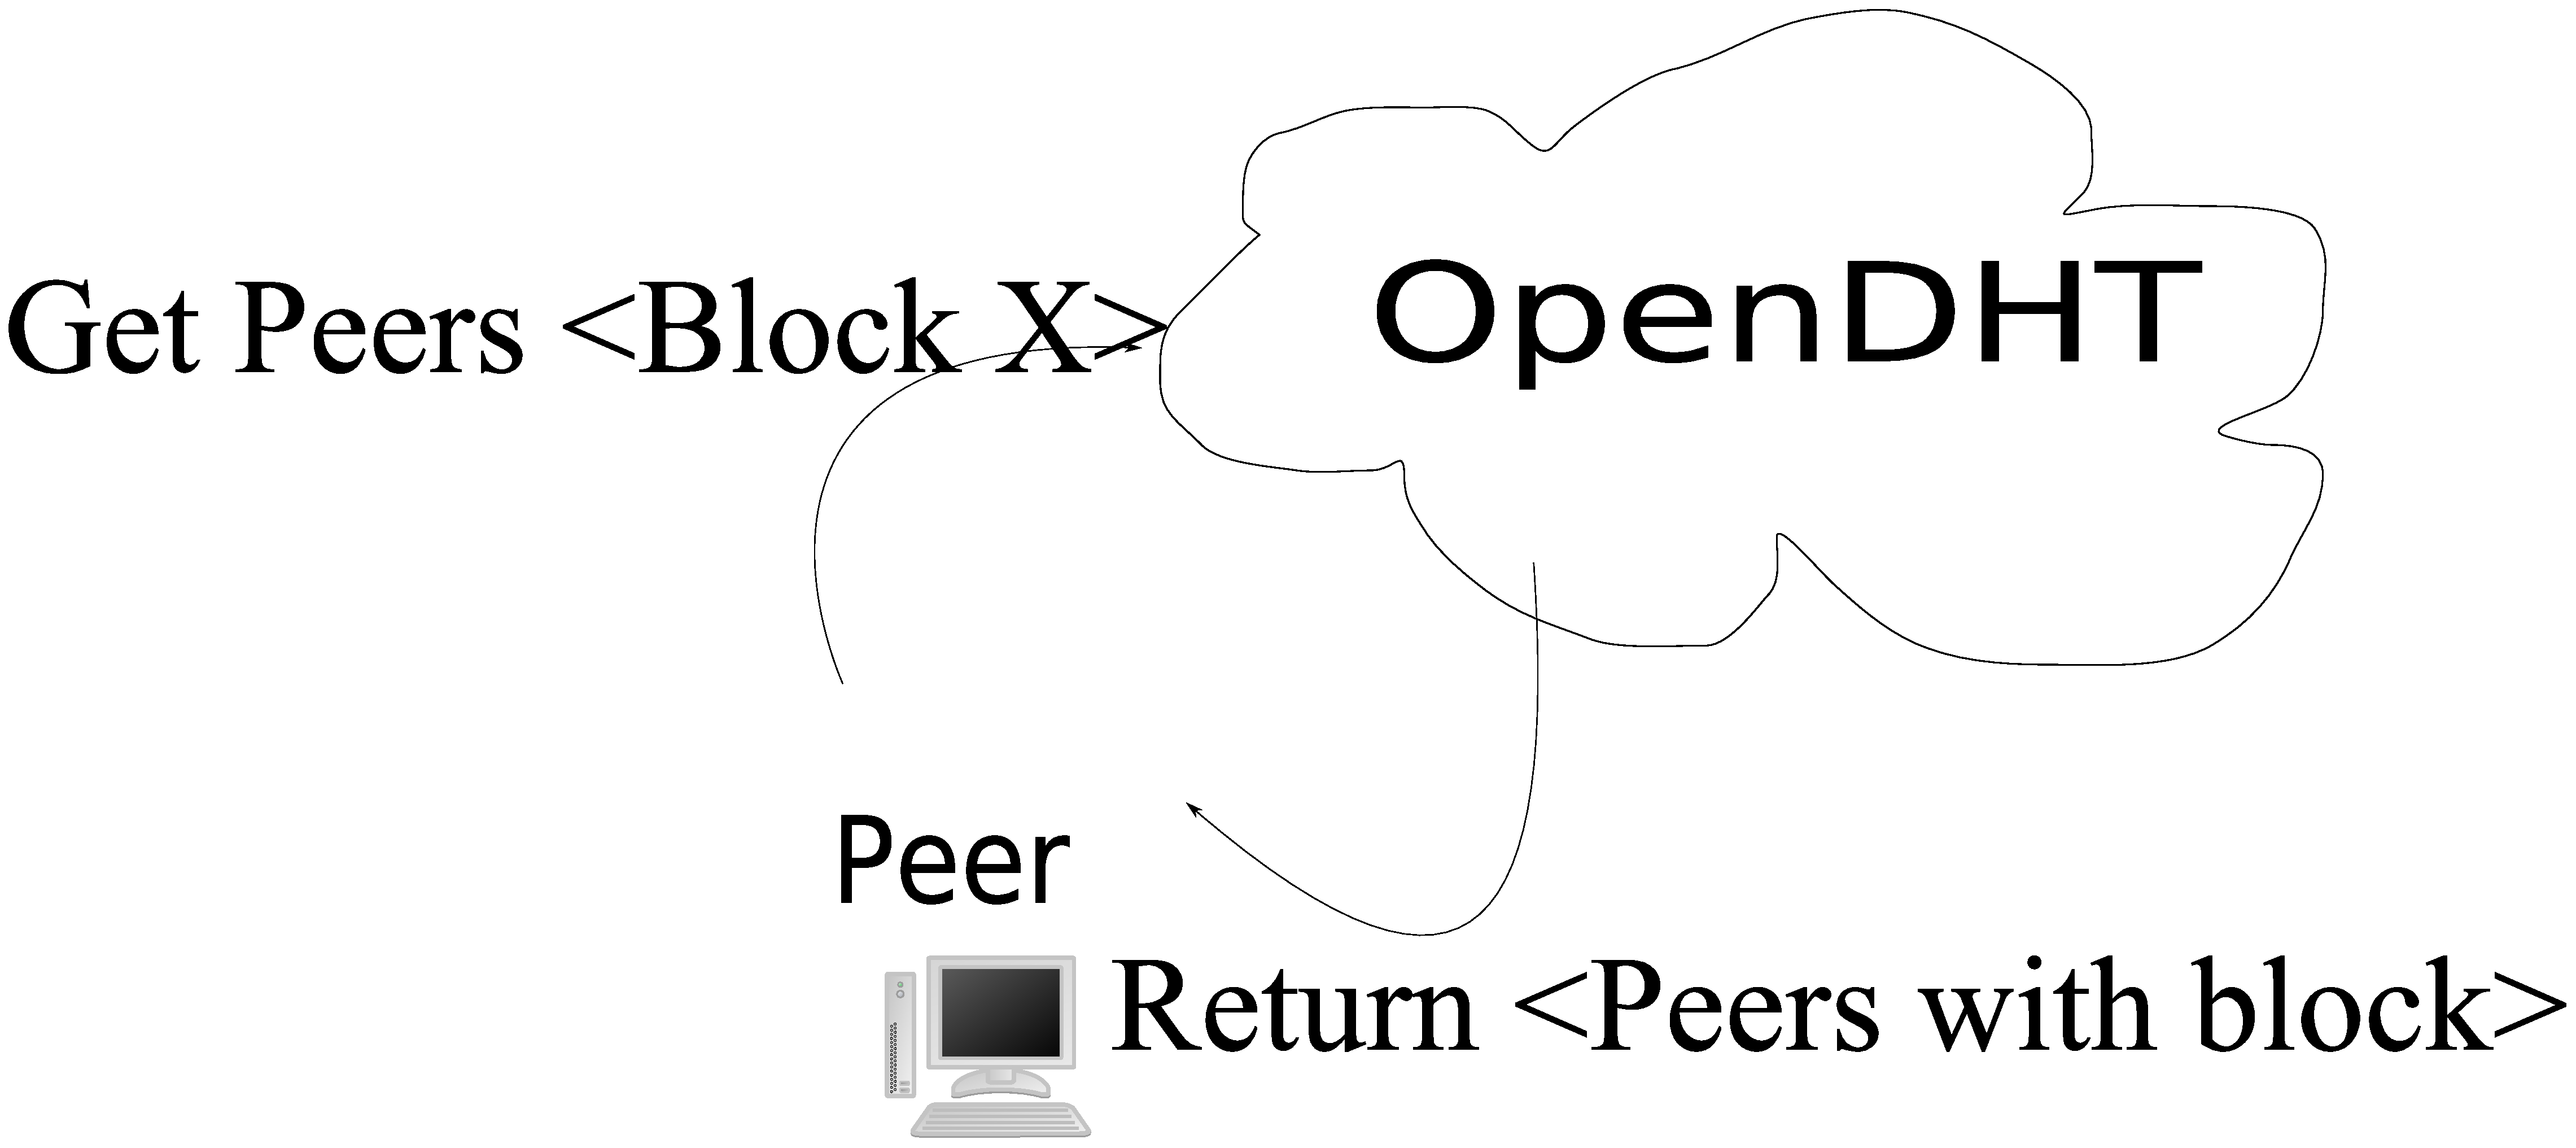
\includegraphics[width=7cm]{pics/peer_step_2.eps}}
    \subfigure[Peer adds itself to list of peers who have that block]{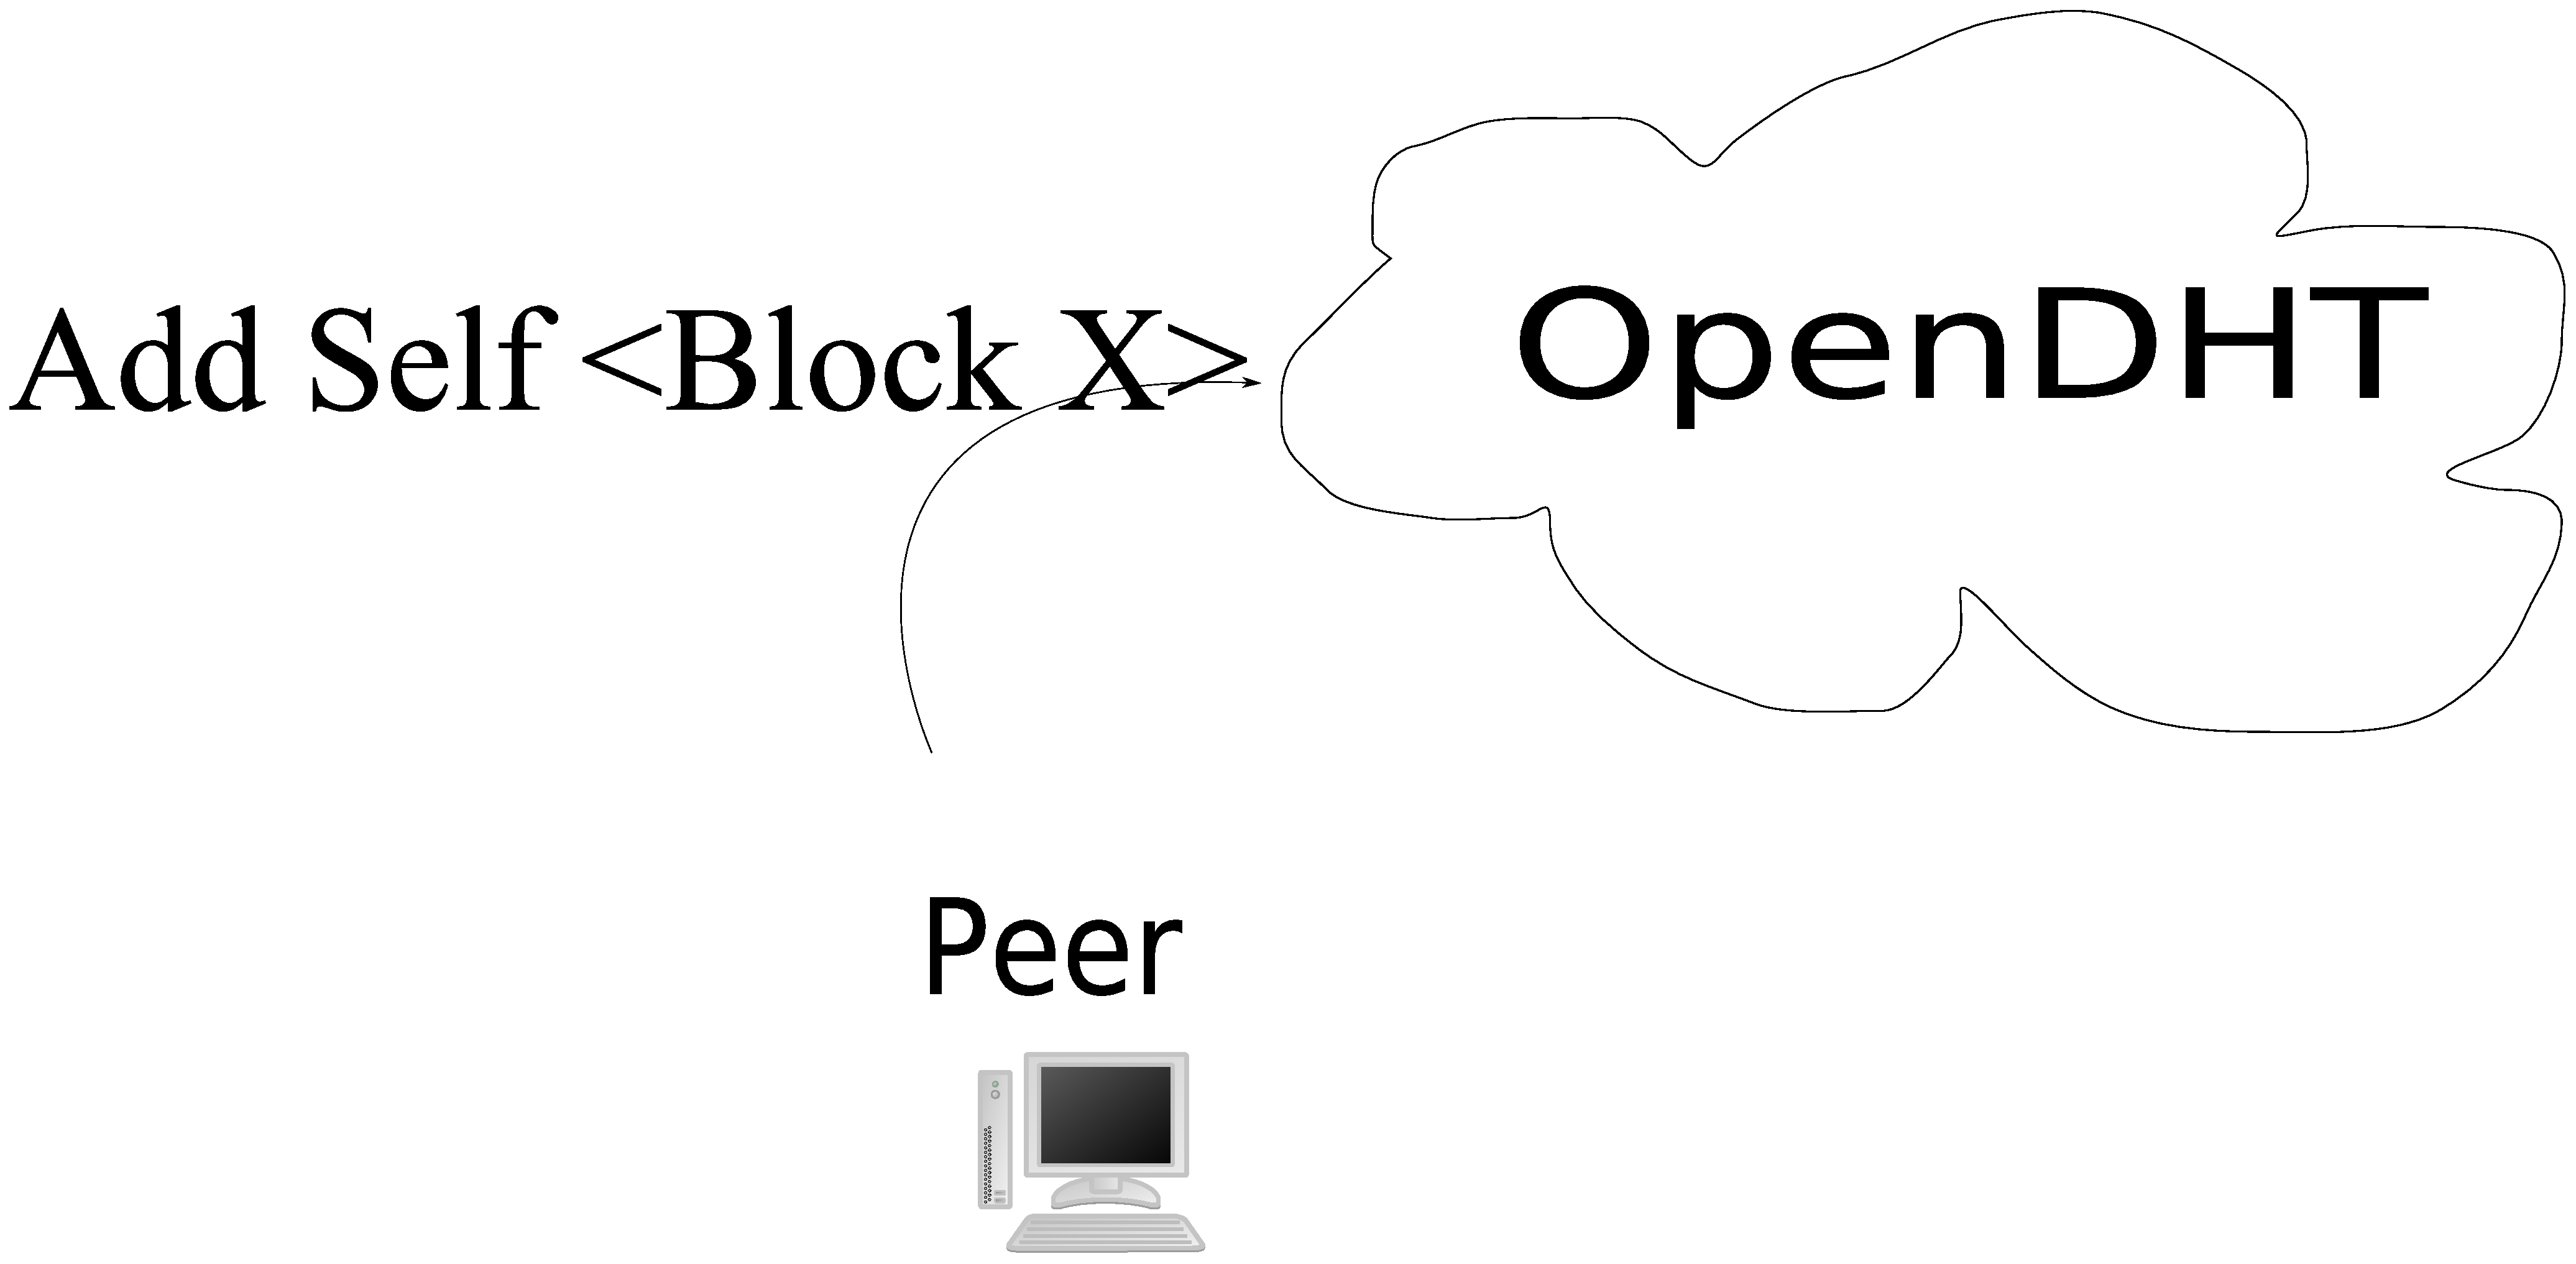
\includegraphics[width=7cm]{pics/peer_step_3.eps}}
    \caption{Steps to accomplish a peer-to-peer-web download.}
    \label{fig:download_all_steps}
  \end{center}
\end{figure*}
